\documentclass{article}

\usepackage{graphicx}
\usepackage{tikz}
\usepackage{tikzsymbols}
\usetikzlibrary{calc,patterns,shapes.geometric}
\pagestyle{empty}
\usepackage[margin=0pt]{geometry}
\geometry{papersize={14in,12in}}

\def\centerarc[#1](#2)(#3:#4:#5){\draw[#1] ($(#2)+({#5*cos(#3)},{#5*sin(#3)})$) arc (#3:#4:#5);}

\begin{document}
	\begin{figure}
		\centering
		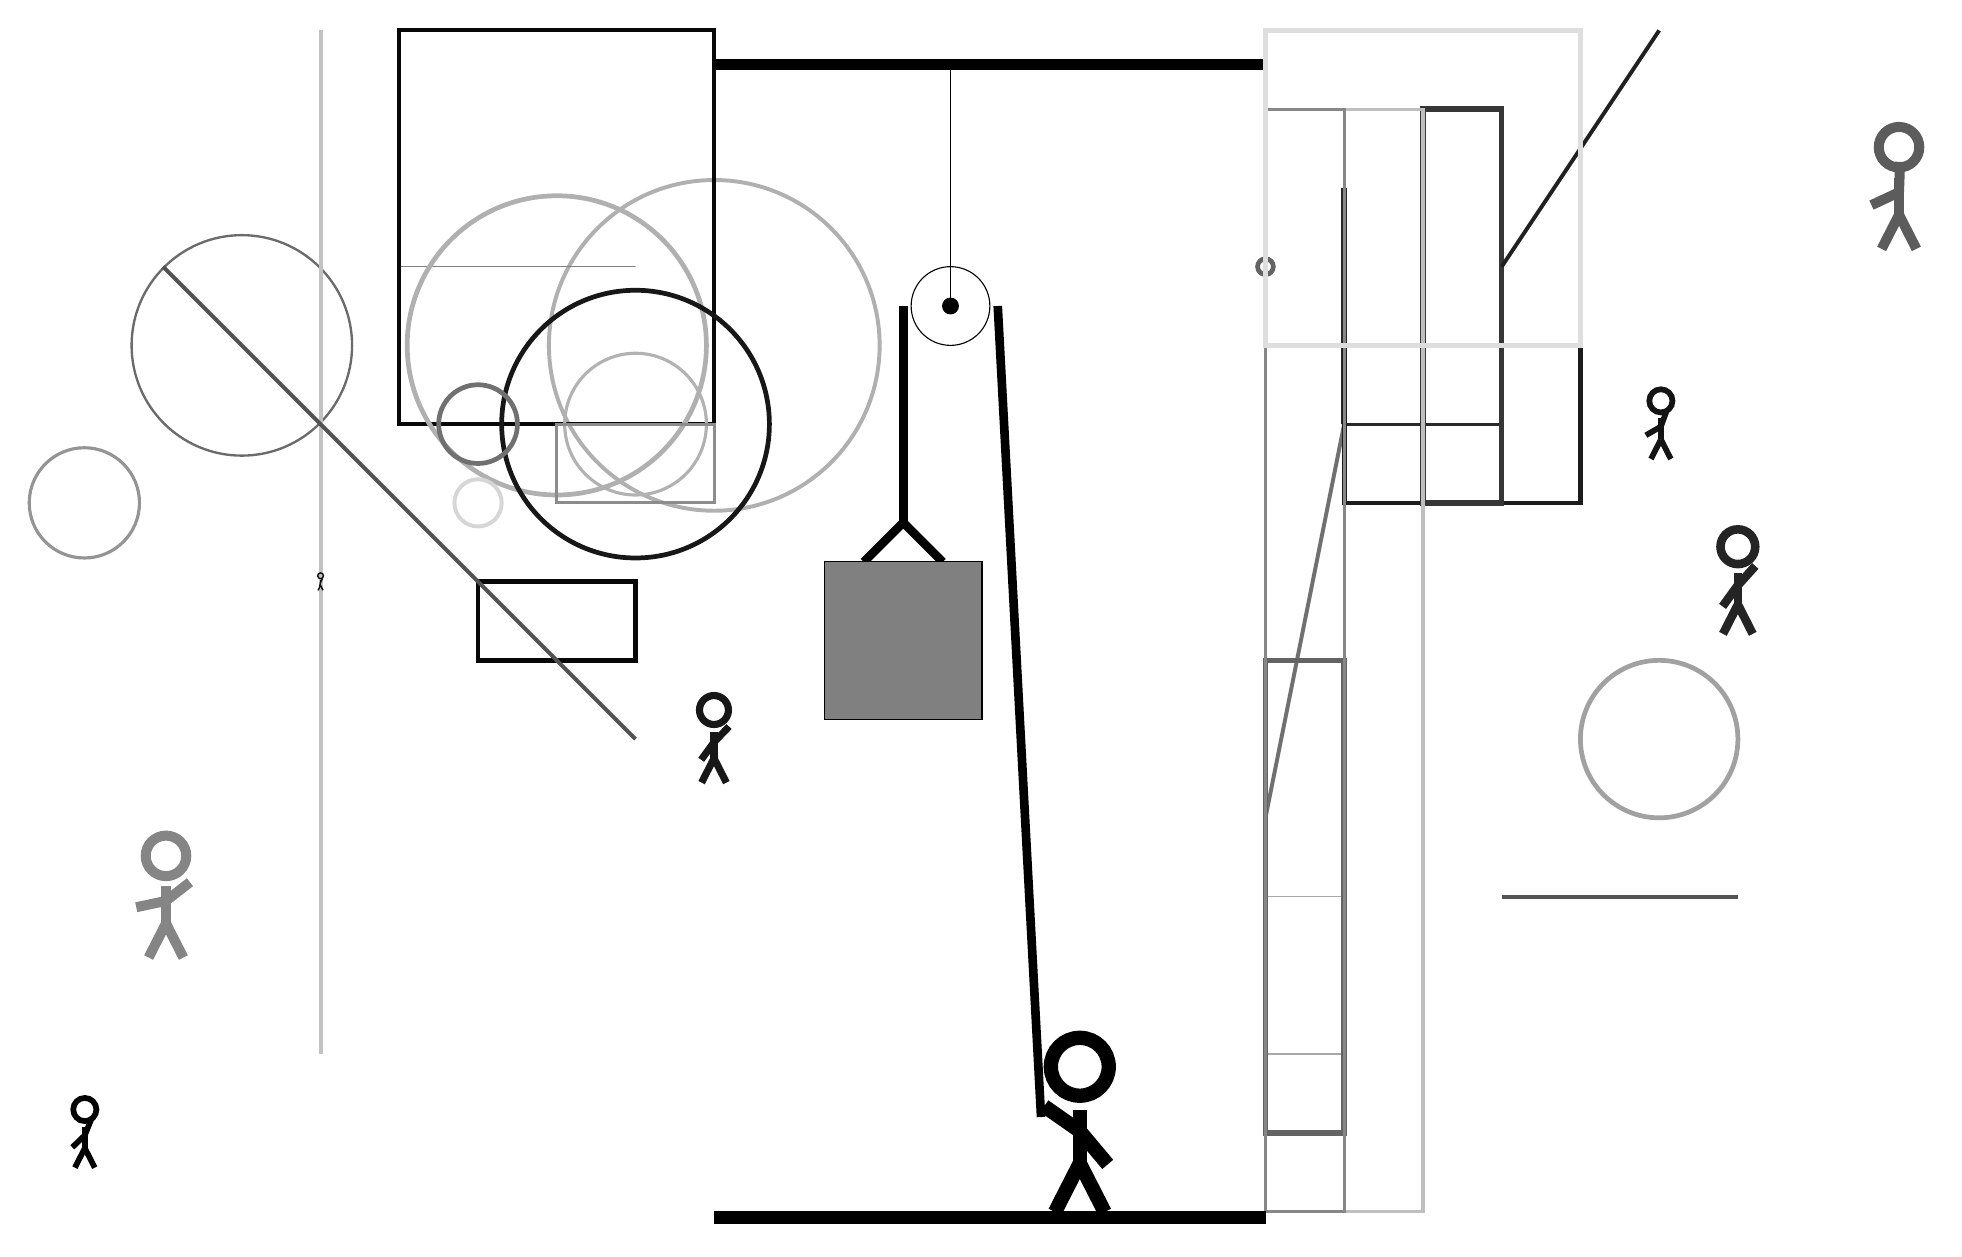
\begin{tikzpicture}
			%%%%% START %%%%%
			
			\draw[fill=black] (-2, 11.5) rectangle (5, 11.625);
			
			\draw (1, 8.5) circle (0.5);
			\draw[fill=black] (1, 8.5) circle (0.1);
			\draw (1, 11.5) -- (1, 8.5);
			
			\draw[line width=1.1mm] (-0.1, 5.25) -- (0.4, 5.75) -- (0.9, 5.25);
			\draw[fill=black!50] (-0.6, 5.25) rectangle (1.4, 3.25);
			
			\draw[line width=1.1mm] (0.4, 8.5) -- (0.4, 5.75);
			\centerarc[line width=1.1mm](1, 8.5)(0:180:0.6);
			\draw[line width=1.1mm](1.6, 8.5) -- (2.15, -1.8);
			
			\draw [line width=0.5mm, color=black!31](-2, 8) circle (2.1);
			
			\draw[line width=0.2mm, color=black!50] (-3, 9) rectangle (-6, 9);
			\draw[line width=0.2mm, color=black!34] (6, -1) rectangle (5, 1);
			\draw[line width=0.5mm, color=black!97] (-2, 7) rectangle (-6, 12);
			\draw [line width=0.3mm, color=black!58](-8, 8) circle (1.4);
			\draw[line width=0.7mm, color=black!84] (6, 10) rectangle (6, 7);
			
			\node[line width=0.4mm, color=black!48] at (-9, 1) {\Strichmaxerl[7][12][38]};
			\draw[line width=0.4mm, color=black!84] (6, 7) rectangle (8, 8);
			\draw[line width=0.5mm, color=black!56](6, 7) -- (5, 2);
			\draw [line width=0.4mm, color=black!42](-10, 6) circle (0.7);
			\node[line width=0.5mm, color=black!92] at (10, 7) {\Strichmaxerl[4][30][70]};
			
			\draw[line width=0.5mm, color=black!24](-7, 12) -- (-7, -1);
			\draw[line width=0.6mm, color=black!89] (6, 6) rectangle (9, 8);
			
			\draw[line width=0.6mm, color=black!97] (-3, 4) rectangle (-5, 5);
			\node[line width=0.3mm, color=black!91] at (-2, 3) {\Strichmaxerl[5][54][46]};
			\draw[line width=0.7mm, color=black!61] (5, 4) rectangle (6, -2);
			
			\draw[line width=0.5mm, color=black!67](8, 1) -- (11, 1);
			\draw [line width=0.4mm, color=black!30](-3, 7) circle (0.9);
			\draw[line width=0.7mm, color=black!79] (7, 6) rectangle (8, 11);
			
			\draw[line width=0.5mm, color=black!87](10, 12) -- (8, 9);
			\draw[line width=0.5mm, color=black!68](-3, 3) -- (-9, 9);
			\draw [line width=0.6mm, color=black!31](-4, 8) circle (1.9);
			\draw [line width=0.6mm, color=black!91](-3, 7) circle (1.7);
			\draw[line width=0.4mm, color=black!25] (5, 11) rectangle (7, -3);
			\draw [line width=0.6mm, color=black!37](10, 3) circle (1.0);
			\node[line width=0.3mm, color=black!93] at (-7, 5) {\Strichmaxerl[1][77][63]};
			
			\draw[line width=0.4mm, color=black!47] (5, -3) rectangle (6, 11);
			\draw [line width=0.6mm, color=black!56](-5, 7) circle (0.5);
			\draw[line width=0.4mm, color=black!45] (-4, 6) rectangle (-2, 7);
			
			\draw [line width=0.5mm, color=black!16](-5, 6) circle (0.3);
			\node[line width=0.4mm, color=black!64] at (13, 10) {\Strichmaxerl[7][25][88]};
			\draw [line width=0.6mm, color=black!61](5, 9) circle (0.1);
			\node[line width=0.2mm, color=black!99] at (-10, -2) {\Strichmaxerl[4][44][68]};
			\draw[line width=0.7mm, color=black!13] (5, 8) rectangle (9, 12);
			\node[line width=0.5mm, color=black!86] at (11, 5) {\Strichmaxerl[6][54][48]};
			
			\node at (2.6, -1.9) {\Strichmaxerl[10][-35][-50]};
			
			\draw[fill=black] (-2, -3) rectangle (5, -3.15);
			
			%%%%% END %%%%%
		\end{tikzpicture}
	\end{figure}	
\end{document}